\documentclass{article}

% Margins.
\setlength{\oddsidemargin}{0in}
\setlength{\evensidemargin}{0in}
\setlength{\headheight}{12pt}
\setlength{\headsep}{42pt}
\setlength{\topmargin}{-54pt}
\setlength{\textwidth}{6.5in}
\setlength{\textheight}{9in}

\usepackage{hyperref}
\usepackage{float}
\usepackage{graphicx}

%opening
\title{Programming for Engineers I\\Lab 02\\Debugging II: Variable Representation and Memory Storage}
\author{Attique Dawood}

\begin{document}

\maketitle

This lab is about representation of integer and floating point numbers. Students will use the debugger to learn exactly how the variables are represented and stored as binary numbers in computer memory\footnotemark.

\footnotetext[1]{It is assumed that students are familiar with Visual Studio and basic debugging functions like starting debugger, single-stepping, adding watches and breakpoints. You can refresh these concepts by referring to the \emph{Debugging} section in \emph{Creating a New Project in Visual Studio}}

\section{Configuration and Platform}
You might have noticed a \verb|Debug| and \verb|Win32| on the Visual Studio toolbar. These are project configuration and solution platform, respectively.
\subsection{Project Configurations}
The project configuration can be of types \verb|Debug| and \verb|Release|. During development stages it is convenient to build/compile in debug mode in order to find and fix bugs. After the development is complete the resulting program is distributed as a \emph{release} version to the end user.
\subsubsection{\texttt{Debug} Configuration}
In debug mode, compiler embeds the built executable with \emph{debugging symbols}. This enables the debugger to read in an executable or binary file and debug it. Without these debugging symbols an executable cannot be debugged. As a result the executable increases in size and will take more time to execute than a normal binary/executable.
\subsubsection{\texttt{Release} Configuration}
An executable/binary file produced in release configuration will be optimized by compiler to run noticeably faster and will be smaller in size than the debug version. The downside is that debugger will not be able to read this file and it cannot be debugged.

\begin{figure}[H]
\centering
\label{Configuration-Platform}
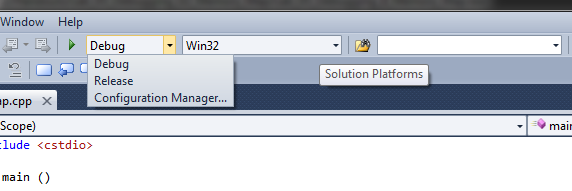
\includegraphics[scale=0.6]{ConfigurationPlatform.png}
\caption{Project configuration and solution platform}
\end{figure}

\subsection{Solution Platform}
\verb|Platform| is the CPU we're trying to target. Normally we only have 32 and 64 bit processors to choose from. Selecting \verb|Win32| will produce a 32 bit executable. Similarly, \verb|x64| can be chosen to compile a 64 bit executable targeting 64 bit processors. Notice, a 64 bit processor can run both 32 and 64 bit executables but a 32 bit processor can only run 32 bit executable files.

\section{Storing Signed/Unsigned Integers and Floating Point Numbers}
It is imperative that you feel comfortable with binary and hexadecimal conversion. Following sections cover a few basic concepts.

\subsection{Binary and Hexadecimal Conversion}
Conversion between binary and hexadecimal notation is straightforward. To convert a binary number, divide it into groups of four bits starting from least significant bit. Add additional zeros to the most significant bit to make the total number of bits a multiple of four. Hexadecimal (or hex) notation is convenient because it saves space. Notice, any number starting with \verb|0x| is a hex value.

\begin{table}[H]
\centering
\label{4-bit-bin-hex-table}
	\begin{tabular}{l c l}
	\hline \hline \\ [-2ex]
	Dec & Bin & Hex\\
	\hline \\ [-2ex]
	0  & 0000 & 0x0\\
	1  & 0001 & 0x1\\
	2  & 0010 & 0x2\\
	3  & 0011 & 0x3\\
	4  & 0100 & 0x4\\
	5  & 0101 & 0x5\\
	6  & 0110 & 0x6\\
	7  & 0111 & 0x7\\
	8  & 1000 & 0x8\\
	9  & 1001 & 0x9\\
	10 & 1010 & 0xA\\
	11 & 1011 & 0xB\\
	12 & 1100 & 0xC\\
	13 & 1101 & 0xD\\
	14 & 1110 & 0xE\\
	15 & 1111 & 0xF\\
	\hline \hline
	\end{tabular}
\caption{4--bit binary--hexadecimal conversion}
\end{table}

\subsection{Storing Unsigned Integers in Memory}
Storing unsigned integers is simple and the procedure is outlined as,
\begin{enumerate}
\item Convert the decimal number to its equivalent binary form.
\item Add 0's before the most significant bit to fill up 32 bits\footnotemark.
\item Divide the number into four bytes. Least significant bit corresponds to first byte and so on.
\item \emph{Lower bytes go to low memory addresses and higher bytes go to high memory addresses.}
\end{enumerate}
\footnotetext[2]{Here 32 bit unsigned integer is assumed because it is the most widely used. Procedure is same for 8, 16 or 64 bit values.}

\subsubsection{Example}
Suppose we want to store an unsigned integer with value 27 at address \verb|0x00000010|.

\begin{verbatim}
27 = 11011 = 00000000000000000000000000011011

     MSB                                     LSB
         00000000 00000000 00000000 00011011
Byte No:     4        3        2        1

Memory Map:
Address       Data(bin) Data(hex)    Byte No
0x00000010    00011011     1B            1
0x00000011    00000000     00            2
0x00000012    00000000     00            3
0x00000013    00000000     00            4
\end{verbatim}


\subsection{2's Complement Notation}
Signed data types like \verb|int| can have negative values. The negative numbers are stored as 2's complement in memory. To calculate 2's complement of a number invert all the bits and add a 1. For example, 0110 (6 in decimal) in inverted form is 1001. By adding 1 we get 1010 which is the 2's complement of 0110. Therefore, -6 would be stored in memory as 1010.

\subsection{Floating Point Numbers}
To review floating point numbers and their conversion please take a look at \url{http://www.tfinley.net/notes/cps104/floating.html} or your class lectures/notes etc. Following example is taken from the above link.
\subsection{Example: Convert 329.390625 to 32 bit Floating Point Notation}
\subsubsection{Compute binary of integral part}
\verb|329 = 101001001|
\subsubsection{Compute binary of fractional part}
This can be done by repeatedly multiplying the fractional part by 2 and examining the bit left of decimal point. Repeat until fractional part becomes zero.
\begin{verbatim}
0.390625* 2 = 0.78125   0
0.78125 * 2 = 1.5625    1
0.5625  * 2 = 1.125     1
0.125   * 2 = 0.25      0
0.25    * 2 = 0.5       0
0.5     * 2 = 1         1
0

329 = 101001001
.390625 = 0110011

329.390625 = 101001001.0110011
\end{verbatim}
\subsubsection{Write the resulting number in scientific notation}
$1.010010010110011 \times 2^8$
\subsubsection{Compute Exponent}
Adding 127 to 8 we get 135. Binary of 135 is \verb|10000111| which is our 8 bit exponent field.
\subsubsection{Write in 32 Floating Point Notation}
Number is positive so sign bit is 0. Exponent was calculated above and mantissa is the fractional part in scientific notation with additional zeros added to make it 23 bits long.
\begin{verbatim}
Sign   Exponent         23 bit Mantissa
0      10000111      01001001011001000000000

Byte Arrangement
MSB                                                  LSB
    0100 0011    1010 0100    1011 0010    0000 0000

Memory Representation
Address    Data(bin)    Data(hex)
base       0000 0000       00
base+1     1011 0010       B2
base+2     1010 0100       A4
base+3     0100 0011       43
\end{verbatim}

\begin{figure}[H]
\centering
\label{Floating-Point-Example}
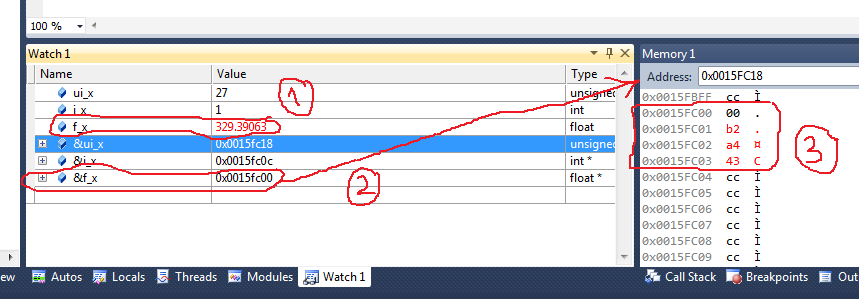
\includegraphics[scale=0.65]{FloatingPointExample.png}
\caption{Using debugger to examine variable data}
\end{figure}

\section{Memory Map in Visual Studio}
\subsection{Configuring Layout}
Figure~\ref{Debugger-Layout} shows a small program in debugger. Notice the layout of debugger and different tabs/windows. At this point we are only interested in two tabs, \verb|Watch| and \verb|Memory|. It is convenient to have these two tabs displayed side-by-side. To add memory window select the right tab (figure\ref{Adding-Memory-Window}) and then navigate to \verb|Debug > Windows > Memory > Memory1|.

\subsection{Memory Contents of Variable}
The example program shown in figure~\ref{Debugger-Layout} has an \verb|unsigned int|, an \verb|int| and a \verb|float| called \verb|ui_x|, \verb|i_x| and \verb|f_x|, respectively. First step is to add these variables to the \verb|Watch| window. Next we need to know their memory addresses in order to access their location in memory. By adding a variable to the watch window with a preceding \verb|&| its address will be displayed. Copy that address into the address location bar on \verb|Memory| window to jump to that memory location. It is convenient to display one or four columns in memory window.

\begin{figure}[H]
\centering
\label{Debugger-Layout}
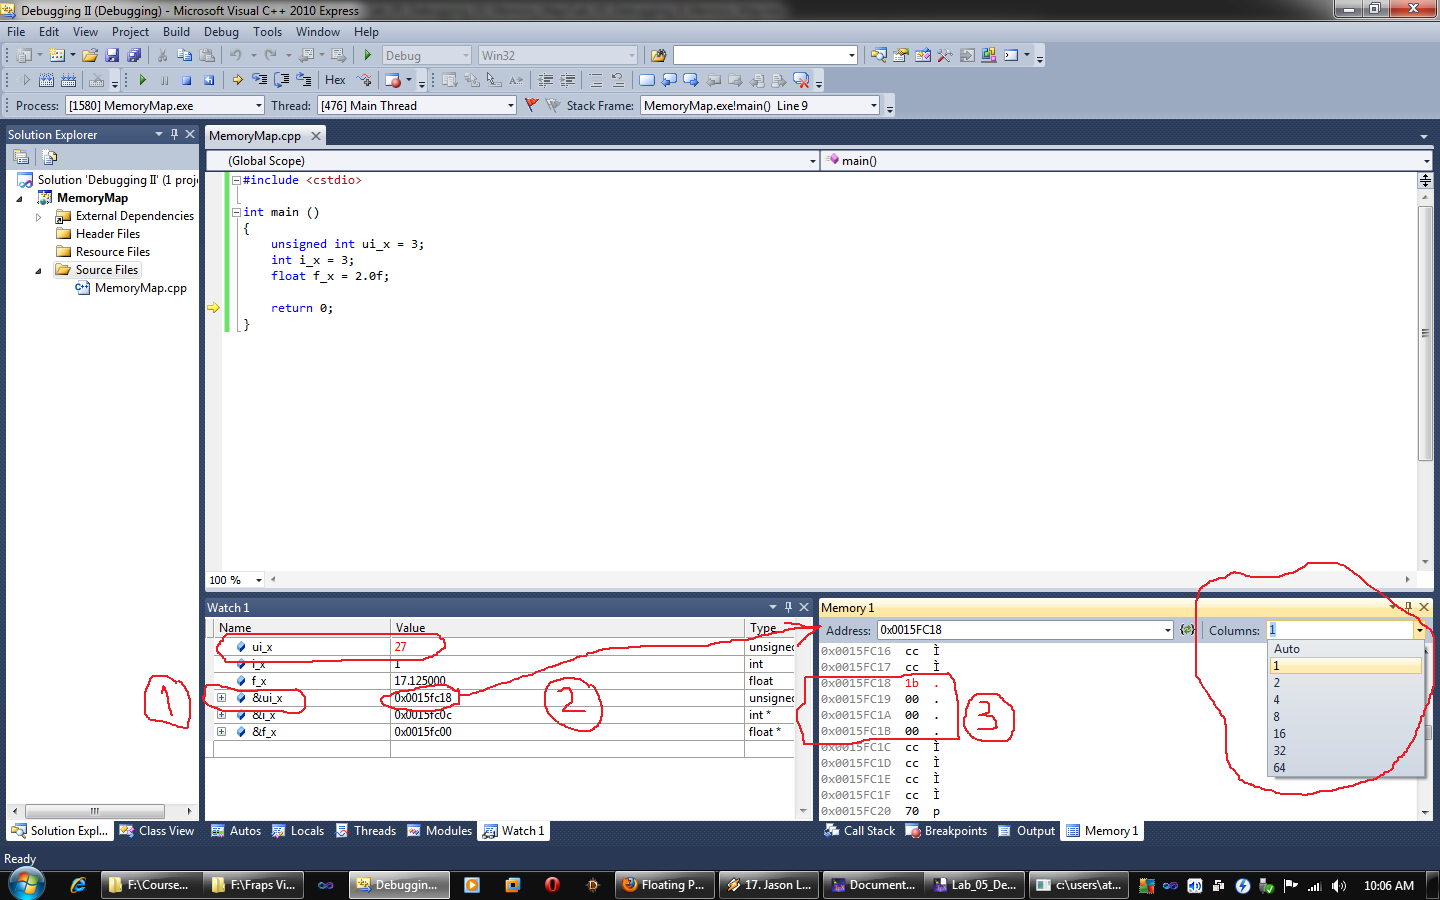
\includegraphics[width=0.95\textwidth]{DebuggerLayout.png}
\caption{Viewing value of a variable in memory}
\end{figure}

\begin{figure}[H]
\centering
\label{Adding-Memory-Window}
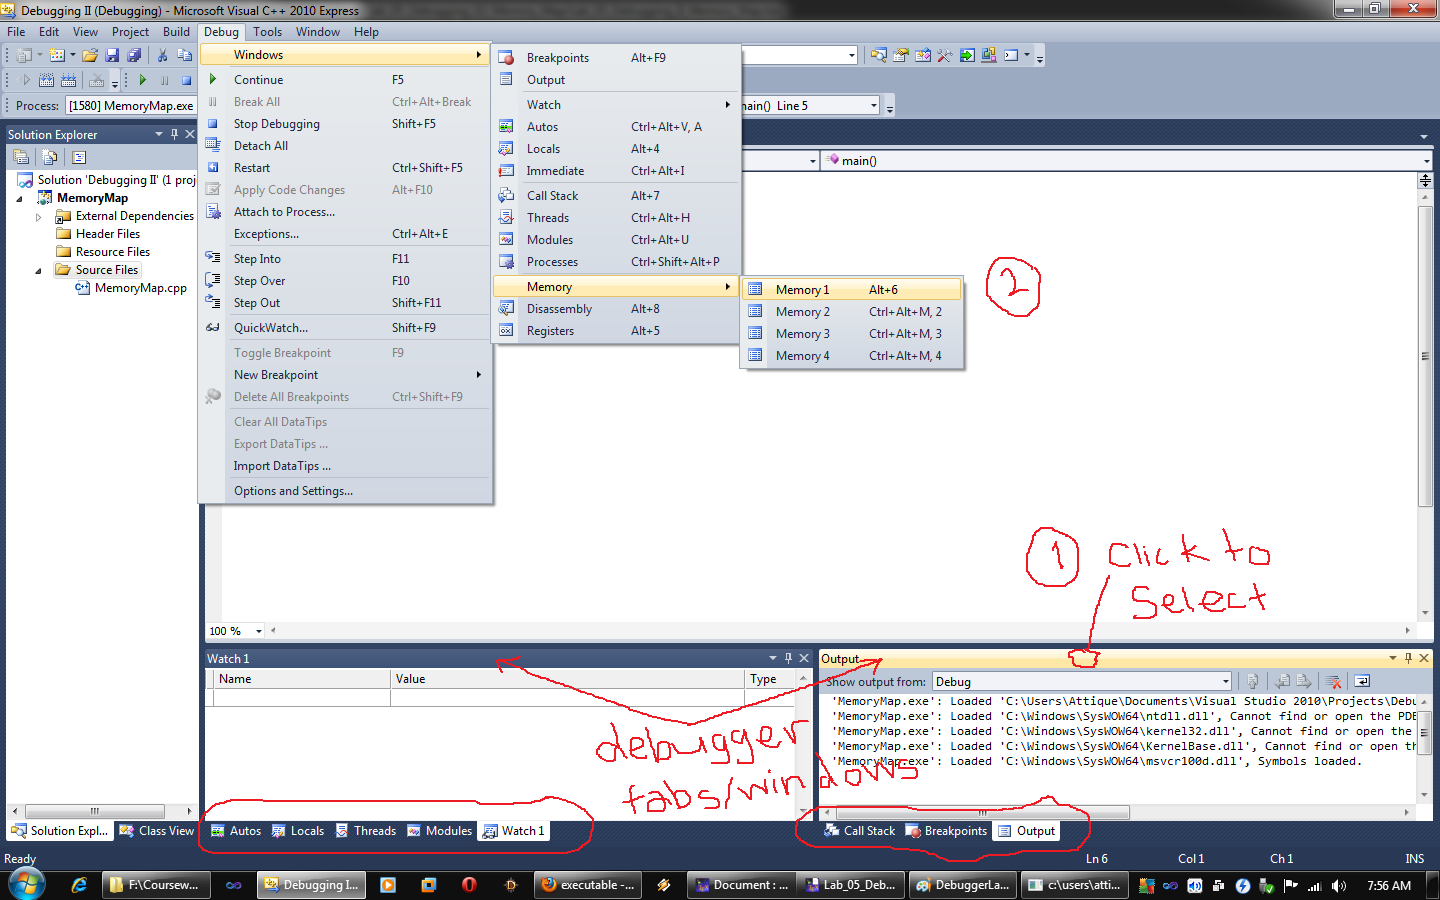
\includegraphics[width=0.95\textwidth]{AddingMemoryWindow.png}
\caption{Adding memory window}
\end{figure}

\section{Exercises}
\textbf{Note: You \emph{must} show all paperwork to get full marks}
\subsection{Unsigned Integers}
Take a random number, for example your roll number. On paper how would this number be stored as an unsigned integer in memory? Does your paperwork match the actual value shown in debugger?
\subsection{Signed Integers}
Repeat the previous exercise assuming the number was negative.
\subsection{Floating Point Notation}
\begin{enumerate}
\item Take your roll number and multiply it with a random number in range 101--999.
\item Divide the resulting number by a random number in range 101-999 such that resulting number has a integral and fractional part. Let's call it \verb|MyFloat|.
\item Convert \verb|Myfloat| into binary.
\item Calculate the 32 bit floating point notation for \verb|MyFloat|.
\item Using debugger, compare your calculated value with actual memory representation.
\end{enumerate}

\end{document}
